\chapter{Implementasi dan Pengujian}
\label{chap:implementation}
Pada bagian ini merupakan rincian atau penjelasan lanjut mengenai lingkungan implementasi perangkat keras maupun perangkat lunak,  serta implementasi program iCalendar Converter dan tampilan antarmukanya. Terakhir akan dibahas mengenai pengujian pada perangkat lunak ini.

\section{Implementasi}
Pada bab ini akan dijabarkan mengenai lingkungan pengembangan perangkat lunak disertai dengan pengujian.

\subsection{Lingkungan Implementasi}
Dalam mengimplementasikan program terdapat dua lingkungan pendukung, yaitu lingkungan perangkat keras dan lingkungan perangkat lunak.
\subsubsection{Lingkungan Perangkat Keras}
Dalam mengembangkan perangkat ini, digunakan spesifikasi perangkat keras sebagai berikut:
\begin{itemize}
	\item \textit{Processor} : Intel Core i7 2.4 Ghz
	\item \textit{Memory} : 8 GB
	\item \textit{Hardisk} : 640 GB
	\item VGA : Nvidia GeForce 540M
	\item \textit{keyboard} dan \textit{mouse standard}
\end{itemize}

\subsubsection{Lingkungan Perangkat Lunak}
Untuk pengembangan perangkat lunak iCalendar Converter, digunakan spesifikasi sebagai berikut:
\begin{itemize}
	\item IDE : Netbeans 8.1
	\item JDK : 1.8 \cite{jdk}
	\item JRE : Java Runtime Enviroment 8 \cite{jdk}
	\item Serta library pihak ketiga seperti JavaFX, Apache POI, dan iCal4j
	\item Editor antarmuka menggunakan SceneBuilder
\end{itemize}

\subsection{Implementasi Program}
Subbab ini menjelaskan tahap dimana program akan dibuat dan dikembangkan dari hasil analisis dan perancangan kelas-kelas maupun \textit{method} yang digunakan. Kode program lengkap dapat dilihat pada Lampiran A. 
Berikut ini merupakan penjelasan kode program dari perangkat lunak iCalendarConverter :
\begin{enumerate}
	\item Kode Program untuk menyimpan jadwal \\
	ScheduleClass merupakan kelas model yang ditujukan untuk menyimpan informasi jadwal yang telah dibaca.\\
	Baris (115-127) kelas ScheduleClass pada lampiran ~\ref{lst:ScheduleClass} menjelaskan tentang penggunaan StringProperty, 
	StringProperty memungkin untuk memberitahu jika ada perubahan pada \textit{variable} tersebut. \textit{Property} membantu untuk menjaga tampilan agar singkron dengan data. Pada ScheduleClass \textit{variable} yang menggunakan StringProperty adalah dosen, subject, dan location.	
	\item Kode program untuk membaca Excel \\
	ExcelConverter merupakan kelas yang dikhususkan untuk membaca excel dan mengeluarkan \textit{output} berupa ArrayList dari kelas model ScheduleClass.\\
	Berikut ini merupakan urutan dari algoritma yang digunakan pada Excel Converter :
\begin{enumerate}
		\item Baris (68-84) pada lampiran ~\ref{lst:ExcelConverter} menjelaskan bagaimana program mencari kolom No. dan Nama Mata Kuliah pada excel. Dua kolom tersebut merupakan acuan data jadwal yang akan dibaca oleh program. Setelah diketahui dimana kolom No. dan Nama Kuliah berada, maka nomer baris dan kolomnya akan dimasukkan kedalam \textit{variable} sebagai acuan membaca program dimulai pada baris itu. Pemilihan kolom No. sebagai acuan dikarenakan isi kolom No. menandakan berapa banyak data jadwal yang ada, sehingga bila isi dari kolom No. bukan angka, maka program akan berhenti membaca. Selanjutnya, pemilihan Nama Mata Kuliah sebagai acuan selain karena data pada kolom itu akan dimasukkan ke kelas model, pun juga karena setelah kolom tersebut terdapat kolom ruang kuliah yang akan dimasukkan kedalam \textit{variable} lokasi pada program.
		Selain itu, nomer kolom ruangan dapat menjadi acuan lokasi dosen mengawas.
		\item Baris (85-87) pada lampiran ~\ref{lst:ExcelConverter} menjelaskan bahwa i sebagai acuan program membaca baris, sedangkan j sebagai acuan program membaca kolom.
		\item Baris (89-93) pada lampiran ~\ref{lst:ExcelConverter} menjelaskan bahwa bila baris ke i program membaca dan isinya kosong maka berhenti membaca.
		\item Baris (96-100) pada lampiran ~\ref{lst:ExcelConverter} menjelaskan bila isi pada kolom No. bukanlah angka dan \textit{blank} maka program berhenti membaca.
		\item Baris (101-107) pada lampiran ~\ref{lst:ExcelConverter} menjelaskan	bila isi kolom No. adalah kosong maka lewati barisnya dan baca baris selanjutnya.
		\item Baris (108-129) pada lampiran ~\ref{lst:ExcelConverter} menjelaskan bahwa bila kolom tersebut adalah tanggal dan jika isinya kosong, maka lewati barisnya. Jika isinya tidak kosong, maka pisahkan isinya menurut tanda "-" dan tanda "," . Lalu, jika ada singkatan Mrt ganti menjadi 3. Jika ada singktan Okt ganti menjadi 10 dan jika ada singkatan 16 maka ganti menjadi 2016. Sehingga format tanggal menjadi 2016-03-01 sebagai contoh. Setelah itu masukan ke \textit{variable} beritipe LocalDate.
		\item Baris (130-163) pada lampiran ~\ref{lst:ExcelConverter} menjelaskan bahwa bila kolom tersebut adalah jam an jika isinya LIBUR maka lewati baris tersebut. Jika isinya Shift maka pasti baris dibawahnya adalah jam. Sehingga, ambil \textit{value} baris dibawahnya, lalu pisahkan menurut tanda "-" dan ganti tanda "." dengan tanda ":" . Kemudian, masukan ke \textit{variable} bertipe LocalTime. Jika isi kolom berisi jam saja, maka pisahkan menurut tanda "-" dan ganti tanda "." dengan tanda ":" . Lalu, masukan ke \textit{variable} bertipe LocalTime.
		\item Baris (164-166) pada lampiran ~\ref{lst:ExcelConverter} menjelaskan bila kolom tersebut adalah Nama Mata Kuliah, maka masukan ke \textit{variable} String Subject.
		\item Baris (173-192) pada lampiran ~\ref{lst:ExcelConverter} menjelaskan bila kolom tersebut adalah ruangan, yang bearti isinya adalah nama dosen yang mengawas. Jika isi kolom diawali dengan Lab, maka pisahkan menurut tanda ":" dan pisahkan kembali menurut tanda ",", sehingga menghasilkan nama dosen saja. Selanjutnya, masukan nama dosen ke ArrayList dosen dan isi ArrayList location dengan kata Lab. Jika isi kolom tidak di awali dengan kata lab, maka masukan nama dosen ke ArrayList dosen dan isi ArrayList location dengan mengambil nomor kolom dari ruangan tersebut dan mencocokannya dengan posisi nama dosen tersebut berada dan isi nomer ruangan kedalam ArrayList Location.
		\item Baris (193-215) pada lampiran ~\ref{lst:ExcelConverter} menjelaskan bahwa karena dua mata kuliah berisikan dua baris kolom dosen yang di \textit{merger} jadi satu dan Apache POI hanya dapat membaca baris pertama kolom yang digabungkan, maka pada baris yang kosong pada ArrayList dosen dan location disi dengan String kosong.
		\item Baris (219-221) pada lampiran ~\ref{lst:ExcelConverter} menjelaskan masukan semua \textit{variable} yang diisikan sebelumnya kedalam sebuah ArrayList ScheduleClass sesuai jumlah ArrayList nama dosen.
		\item Baris (222-223) pada lampiran ~\ref{lst:ExcelConverter} menjelaskan hapus semua isi ArrayList dosen agar tidak ada duplikasi.
		\item Baris (227) pada lampiran ~\ref{lst:ExcelConverter} menjelaskan hasil ArrayList method Converter() akan kembali dicek oleh \textit{method} mergering().
		\item Baris (235-242) pada lampiran ~\ref{lst:ExcelConverter} menjelaskan jika ada dosen yang isinya kosong pada ArrayList ScheduleList, maka pindahkan isinya ke ArrayList baru yang bernama ScheduleListSmt.
		\item Baris (243-250) pada lampiran ~\ref{lst:ExcelConverter} menjelaskan cara menghapus isi ArrayList ScheduleList yang sama dengan ArrayList SchedulelistSmt.
		\item Baris (251-263) pada lampiran ~\ref{lst:ExcelConverter} menjelaskan jika tanggal dan jam pada ArrayList ScheduleList sama dengan ArrayList ScheduleListSmt, maka tambahkan subject dari ArrayList ScheduleList dengan subject yang ada di ArrayList ScheduleListSmt.
		\item Baris (264) pada lampiran ~\ref{lst:ExcelConverter} menjelaskan kembalian ArrayList ScheduleList.				
	\end{enumerate}

\item Kode Program untuk Konversi Kalendar \\
Kelas CalendarConverter merupakan kelas yang dikhususkan untuk mengkonversi ScheduleClass menjadi file iCalendar. \\
Berikut ini penjelasan dari implementasi kelas CalendarConverter :
\begin{enumerate}
	\item Baris (41-43) pada lampiran ~\ref{lst:CalendarConverter} menjelaskan pembuatan \textit{timeZone} untuk wilayah Indonesia.
	\item Baris (46-52) pada lampiran ~\ref{lst:CalendarConverter} menjelaskan pembuatan tanggal dan waktu dimulainya ujian dengan mengkonversi tahun, bulan, tanggal, jam, dan menit dari ScheduleClass.
	\item Baris (55-61) pada lampiran ~\ref{lst:CalendarConverter} menjelaskan pembuatan tanggal dan waktu ujian tersebut berakhir dengan mengkonversi tahun, bulan, tanggal, jam, dan menit dari ScheduleClass.
	\item Baris (65-72) pada lampiran ~\ref{lst:CalendarConverter} menjelaskan pembuatan \textit{event} pada kalendar.
	\item Baris (80) pada lampiran ~\ref{lst:CalendarConverter} memasukan timeZone pada kalendar.
	\item Baris (83-85) pada lampiran ~\ref{lst:CalendarConverter} menjelaskan identitas pembuat calendar.
	\item Baris (89-92) pada lampiran ~\ref{lst:CalendarConverter} menjelaskan cara pembuatan calendar.
	\item Baris (95-96) pada lampiran ~\ref{lst:CalendarConverter} memasukan \textit{event} yang telah dibuat kedalam kalendar dan \textit{print} sesudahnya.
	\item Baris (99-105) pada lampiran ~\ref{lst:CalendarConverter} menjelaskan cara menyimpan file iCalendar pada direktori tertentu.
\end{enumerate}

\item Kode Program \textit{Controller} \\
Kelas FXMLDocumentController merupakan kelas yang bertugas menjadi penghubung kelas \textit{view} dengan kelas-kelas lainnya. Di kelas ini hasil dari excel yang telah dibaca akan ditampilkan pada tabelview dan semua fungsi \textit{button} dan  \textit{textbox} di atur dalam kelas ini. \\
Berikut ini penjelasan dari kode-kode dalam kelas FXMLDocumentController :
\begin{enumerate}
	\item Baris (55-58) pada lampiran ~\ref{lst:FXMLDocumentController} menjelaskan file yang akan dipilih nanti harus berekstensi .xlsx.
	\item Baris (59) pada lampiran ~\ref{lst:FXMLDocumentController} menjelaskan bagaimana memunculkan \textit{pop-up window} untuk memilih file \textit{input}.
	\item Baris (61-68) pada lampiran ~\ref{lst:FXMLDocumentController} menjelaskan jika file tidak kosong maka ambil \textit{path}file tersebut dan isikan \textit{textbox browse} dengan \textit{path} file tersebut.
	\item Baris (74-75) pada lampiran ~\ref{lst:FXMLDocumentController} menjelaskan konversi file excel tersebut, kemudian ambil hasilnya dan masukan kedalam ObservableArrayList.
	\item Baris (78-84) pada lampiran ~\ref{lst:FXMLDocumentController} menjelaskan cara menampilkan hasil konversi kedalam \textit{tableview} dengan mengisikan sesuai urutan kolom pada \textit{tableview}.
	\item Baris (86-95) pada lampiran ~\ref{lst:FXMLDocumentController} menjelaskan masukan semua ObservableArrayList jadwalList kedalam ObservableArrayList filteredData untuk keperluan filter nanti dan jika ada perubahan pada ObservableArrayList jadwalList maka \textit{update} pula ObservableArrayList filteredData.
	\item Baris (108) pada lampiran ~\ref{lst:FXMLDocumentController} menjelaskan ambil kelas ScheduleClass yang dipilih oleh \textit{user} dan masukan kedalm \textit{variable} selected.
	\item Baris (111-112) pada lampiran ~\ref{lst:FXMLDocumentController} menjelaskan bahwa setiap file yang akan disimpan diberikan ekstensi .ics .
	\item Baris (113) pada lampiran ~\ref{lst:FXMLDocumentController} menjelaskan cara memunculkan \textit{save dialog}.
	\item Baris (117-126) pada lampiran ~\ref{lst:FXMLDocumentController} menjelaskan ambil path direktori dimana \textit{user} akan menyimpan file, lalu konversi jadwal yang telah dipilih oleh \textit{user} dan simpan di direktori yang sudah ditentukan.
	\item Baris (131-140) pada lampiran ~\ref{lst:FXMLDocumentController} menjelaskan jika \textit{textbox filter} di isi oleh \textit{user} maka jadwal di tabel pun berubah sesuai dengan nama dosen yang di tuliskan \textit{user}.
	\item Baris (145-154) pada lampiran ~\ref{lst:FXMLDocumentController} menjelaskan cara \textit{update} filteredData sesuai nama dosen yang di input oleh \textit{user}.
	\item Baris (158-170) pada lampiran ~\ref{lst:FXMLDocumentController} menjelaskan bila nama dosen yang ditulis di \textit{textbox} filter sama dengan nama dosen yang ada di ScheduleClass, maka kembalikan nilai \textit{true}. Jika tidak, maka kembalikan nilai \textit{false}.
	\item Baris (175-177) pada lampiran ~\ref{lst:FXMLDocumentController} menjelaskan pengurutan kembali tabel, sehingga isi tabelnya sesuai dengan apa yang di masukan pada \textit{textboxt} oleh \textit{user} sebelumnya.
\end{enumerate}
	
\end{enumerate}

\section{Implementasi Antarmuka}
Pada subbab ini akan dibahas implementasi antarmuka dari perangkat lunak. Terdapat beberapa perubahan dari perancangan antarmuka perangkat lunak pada bab 4.\\ 
Berikut ini implementasi antarmuka dari perangkat lunak iCalendarConverter :
\begin{enumerate}
	\item Tampilan perangkat lunak iCalendarConverter
		\begin{figure}[H]
		\centering
		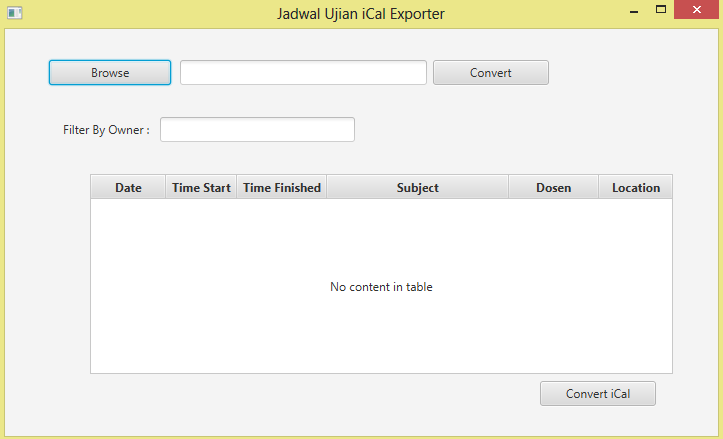
\includegraphics[scale=0.7]{Gambar/implementAntarmuka}
		\caption{Tampilan antarmuka perangkat lunak}
		\label{fig:implementAntarmuka}
		\end{figure}
		Pada tampilan \ref{fig:implementAntarmuka} terlihat beberapa perubahan dengan perancangan antarmuka pada bab sebelumnya. Beberapa perubahan tersebut diantaranya, fungsi fitur \textit{download} yang terletak pada tabel digantikan dengan \textit{button} Convert to iCal pada antarmuka. Hal ini dikarenakan sangat sulit untuk membuat \textit{button} pada setiap isi dari tabel yang berbeda-beda isinya. Selain itu, jika setiap isi tabel mempunyai file iCal akan sangat memakan memori apalagi jika jumlah datanya sangat banyak. Maka, diputuskan untuk membuat satu \textit{button} Convert to iCal yang menangkap \textit{selected item} dari kursor pengguna pada tabel. Selanjutnya, jika pengguna menekan tombol tersebut akan memunculkan \textit{pop-up window} meminta pengguna menentukan tempat penyimpanan file iCal dari jadwal yang telah dipilih sebelumnya.     
	\item Tampilan Antarmuka ketika file excel jadwal mengawas telah dimasukkan
		\begin{figure}[H]
		\centering
		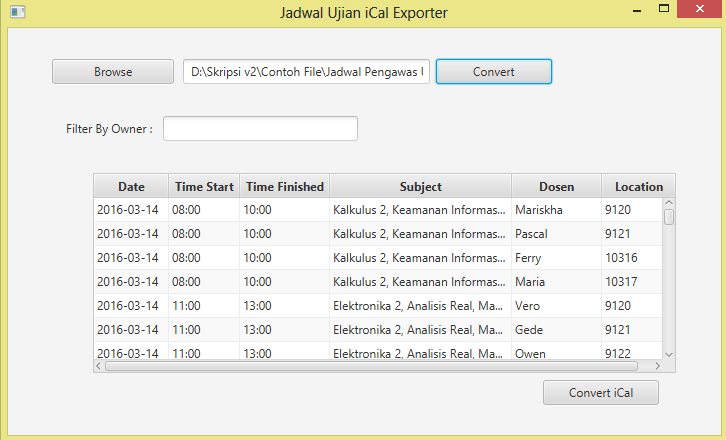
\includegraphics[scale=0.7]{Gambar/implementAntarmuka2}
		\caption{Tampilan antarmuka setelah file mengawas dimasukkan}
		\label{fig:implementAntarmuka}
		\end{figure}
\end{enumerate}

\section{Pengujian}
Pada subbab ini akan dilakukan pengujian pada perangkat lunak untuk mengetahui apakah program dapat berjalan sesuai dengan apa yang di inginkan. Terdapat dua pengujian yaitu :
\begin{enumerate}
	\item Pengujian Fungsional.
	\item Pengujian Eksperimental.
\end{enumerate}

\subsection{Pengujian Fungsional}
Pada pengujian ini akan di uji mengenai fungsionalitas dari perangkat lunak. Selain itu, dalam pengujian fungsional menggunakan file uji \ref{fig:formatLama} untuk mengetahui apakah program berjalan sesuai harapan dan beberapa fungsi berjalan dengan baik. Berikut hasil pengujiannya : 
\begin{table}[H]
	\centering
		\caption{Tabel hasil pengujian fungsional}
		\label{tab:fungsional}
		\begin{tabular}{ | p{4cm} | p{4cm} | c | }
			\hline
				Hal yang diuji & Hasil yang diharapkan & Hasil \\ \hline
				Browse file excel & PL dapat melakukan browse file excel & Berhasil \ref{fig:browseFile}\\ \hline
				Path file excel & PL dapat menangkap alamat file dari \textit{input file} excel & Berhasil \ref{fig:pathFile} \\ \hline
				Menampilkan Jadwal ke layar & PL menampilkan ke layar file excel yang telah dibaca & Berhasil \ref{fig:jadwalKeLayar} \\ \hline
				Konversi ke iCal & PL dapat mengkonversi jadwal yang diseleksi pengguna kedalam iCalendar & Berhasil \ref{fig:konversiiCal} \\ \hline
				Filter nama dosen & PL dapat menampilkan nama dosen yang telah di filter, sesuai yang di yang dimasukkan oleh pengguna pada \textit{textbox} filter & Berhasil \ref{fig:filterDosen} \\ \hline
				Hasil Filter dapat dikonversi ke iCal & Hasil Filter pada PL dan diseleksi oleh pengguna, dapat di konversikan kedalam iCal & Berhasil \ref{fig:filterKonvertiCal} \\ \hline
				\textit{Import} Google Calendar & Hasil konversi PL dapat di masukan kedalam Google Calendar & Berhasil \ref{fig:importGC} \\ \hline
				Dapat dibuka di Outlook & Hasil konversi PL dapat di buka di Outlook & Berhasil  \ref{fig:hasilOutlook}\\ \hline
				Hasil filter dapat di \textit{import} Google Calendar & Hasil filter konversi PL dapat di masukan kedalam Google Calendar & Berhasil \ref{fig:importGCFilter} \\ \hline
				Hasil filter Dapat dibuka di Outlook & Hasil filter konversi PL dapat di buka di Outlook & Berhasil \ref{fig:hasilOutlookFilter} \\ \hline
		\end{tabular}
\end{table}

Berikut ini adalah tampilan dari hasil pengujian yang telah dilakukan pada tabel ~\ref{tab:fungsional} :

		\begin{figure}[H]
		\centering
		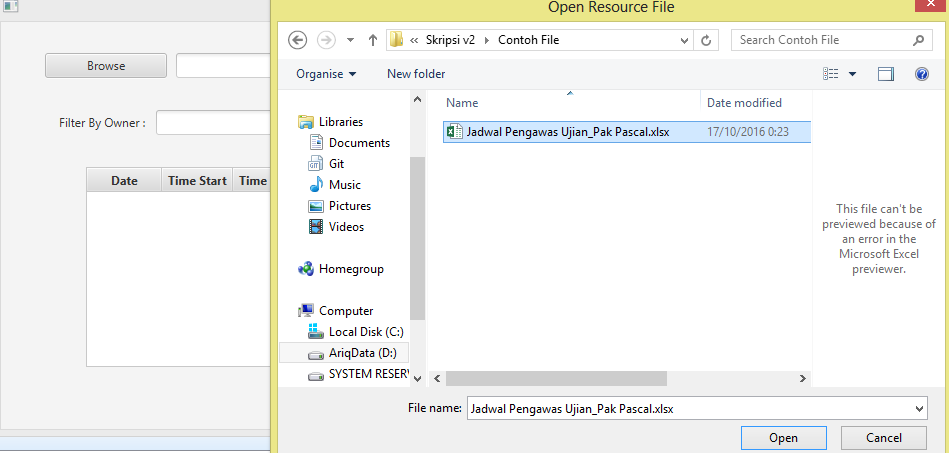
\includegraphics[scale=0.7]{Gambar/browseFile}
		\caption{Tampilan browse file excel mengawas ujian}
		\label{fig:browseFile}
		\end{figure}

		\begin{figure}[H]
		\centering
		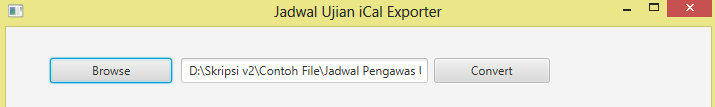
\includegraphics[scale=0.8]{Gambar/pathFile}
		\caption{Tampilan path file excel mengawas ujian}
		\label{fig:pathFile}
		\end{figure}

		\begin{figure}[H]
		\centering
		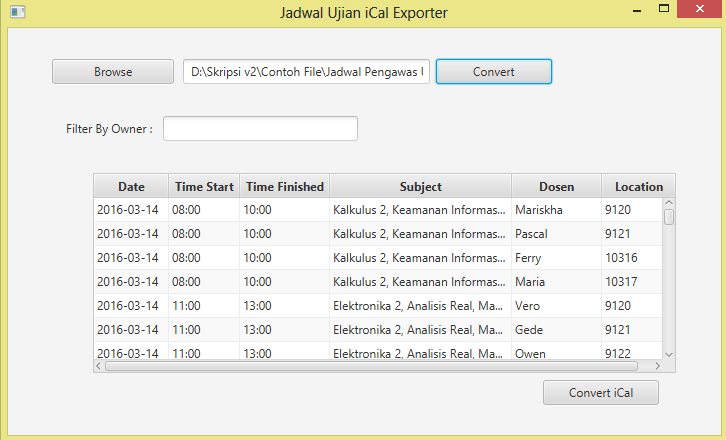
\includegraphics[scale=0.7]{Gambar/implementAntarmuka2}
		\caption{PL menampilkan jadwal ke layar}
		\label{fig:jadwalKeLayar}
		\end{figure}

		\begin{figure}[H]
		\centering
		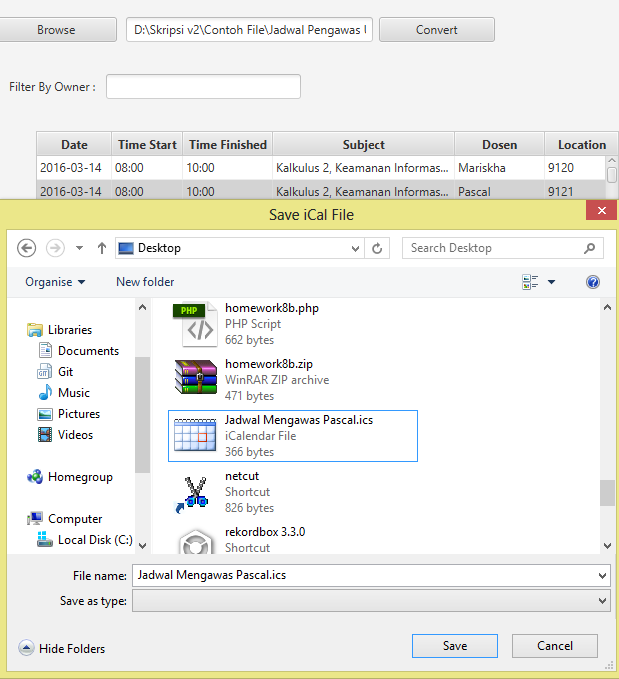
\includegraphics[scale=0.6]{Gambar/konversiiCal}
		\caption{PL mengkonversi jadwal ke format iCal}
		\label{fig:konversiiCal}
		\end{figure}
		
		\begin{figure}[H]
		\centering
		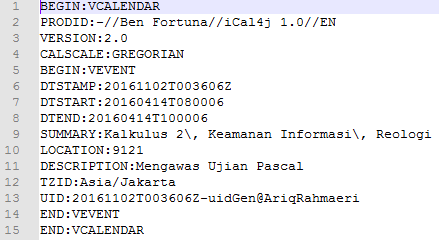
\includegraphics[scale=0.8]{Gambar/fileiCal}
		\caption{File iCal}
		\label{fig:fileiCal}
		\end{figure}

		\begin{figure}[H]
		\centering
		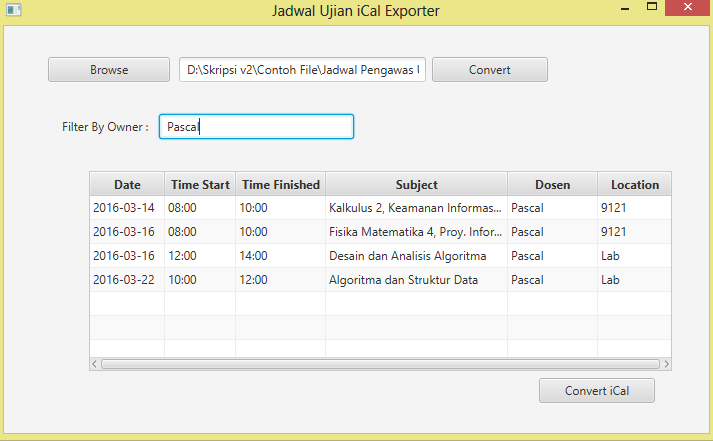
\includegraphics[scale=0.7]{Gambar/filterDosen}
		\caption{Hasil pengujian filter nama dosen}
		\label{fig:filterDosen}
		\end{figure}

		\begin{figure}[H]
		\centering
		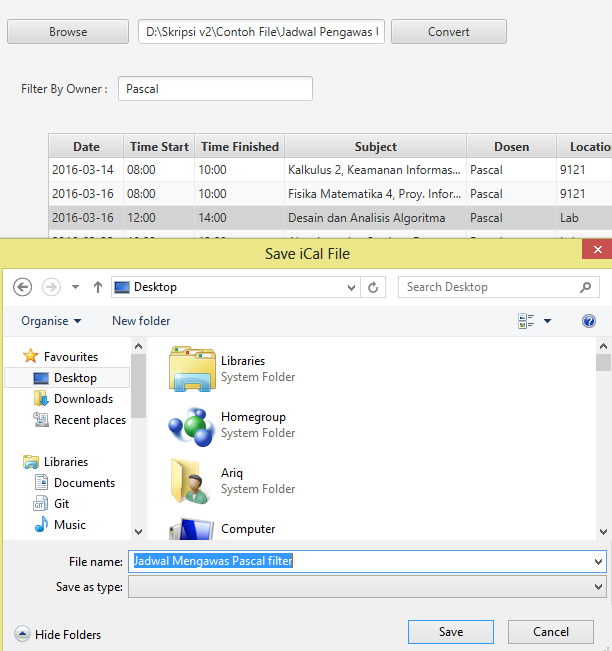
\includegraphics[scale=0.6]{Gambar/filterKonvertiCal}
		\caption{Hasil pengujian convert hasil filter kedalam iCal}
		\label{fig:filterKonvertiCal}
		\end{figure}
		
		\begin{figure}[H]
		\centering
		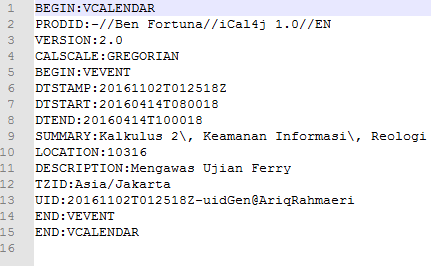
\includegraphics[scale=0.7]{Gambar/fileiCalFilter}
		\caption{File iCal Filter}
		\label{fig:fileiCalFilter}
		\end{figure}
	
 
		\begin{figure}[H]
		\centering
		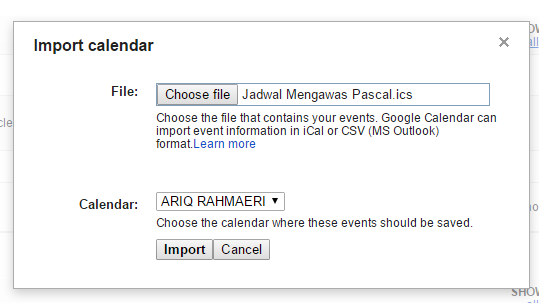
\includegraphics[scale=0.8]{Gambar/importGC}
		\caption{Hasil pengujian import kedalam Google Calendar}
		\label{fig:importGC}
		\end{figure}
		
		\begin{figure}[H]
		\centering
		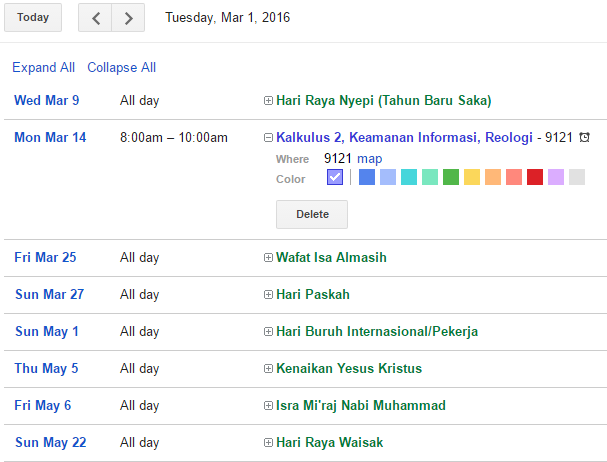
\includegraphics[scale=0.7]{Gambar/hasilGC}
		\caption{Hasil import ke Google Calendar}
		\label{fig:hasilGC}
		\end{figure}
		
		\begin{figure}[H]
		\centering
		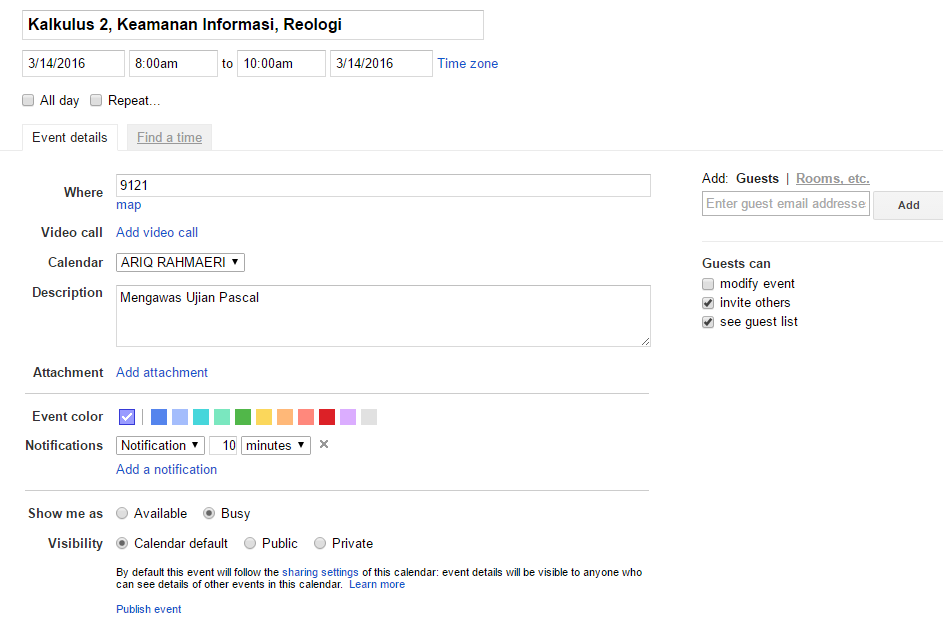
\includegraphics[scale=0.5]{Gambar/hasilGC2}
		\caption{Hasil import ke Google Calendar bagian 2 }
		\label{fig:hasilGC2}
		\end{figure}
		

			\begin{figure}[H]
			\centering
			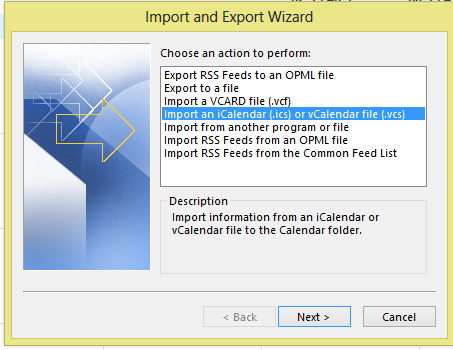
\includegraphics[scale=0.8]{Gambar/importOutlook}
			\caption{\textit{Import} file iCal kedalam MS Outlook }
			\label{fig:importOutlook}
			\end{figure}
		
			\begin{figure}[H]
			\centering
			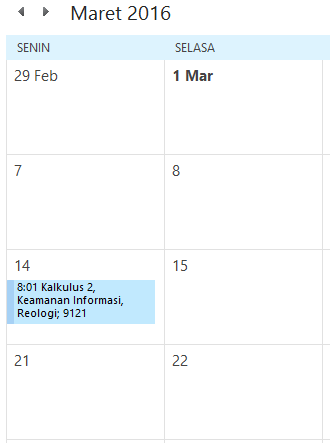
\includegraphics[scale=0.8]{Gambar/hasilOutlook2}
			\caption{File hasil Konversi berada pada kalender MS Outlook }
			\label{fig:hasilOutlook2}
			\end{figure}
			
			\begin{figure}[H]
			\centering
			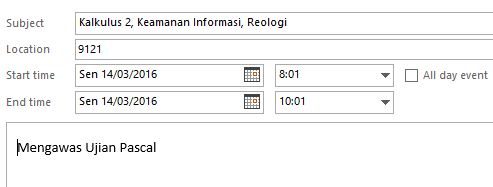
\includegraphics[scale=0.8]{Gambar/hasilOutlook}
			\caption{File hasil Konversi dapat dibuka di MS Outlook }
			\label{fig:hasilOutlook}
			\end{figure}
		

			\begin{figure}[H]
			\centering
			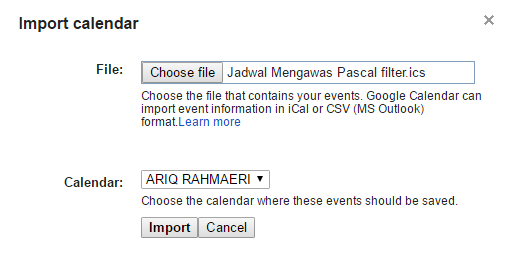
\includegraphics[scale=0.8]{Gambar/importGCFilter}
			\caption{Hasil pengujian import file yang di filter kedalam Google Calendar }
			\label{fig:importGCFilter}
			\end{figure}
			
			\begin{figure}[H]
			\centering
			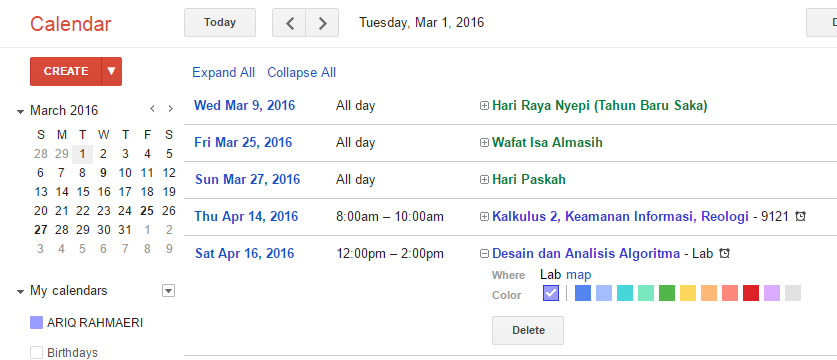
\includegraphics[scale=0.7]{Gambar/hasilGCFilter}
			\caption{Hasil import file yang di filter ke Google Calendar}
			\label{fig:hasilGCFilter}
			\end{figure}
			
			\begin{figure}[H]
			\centering
			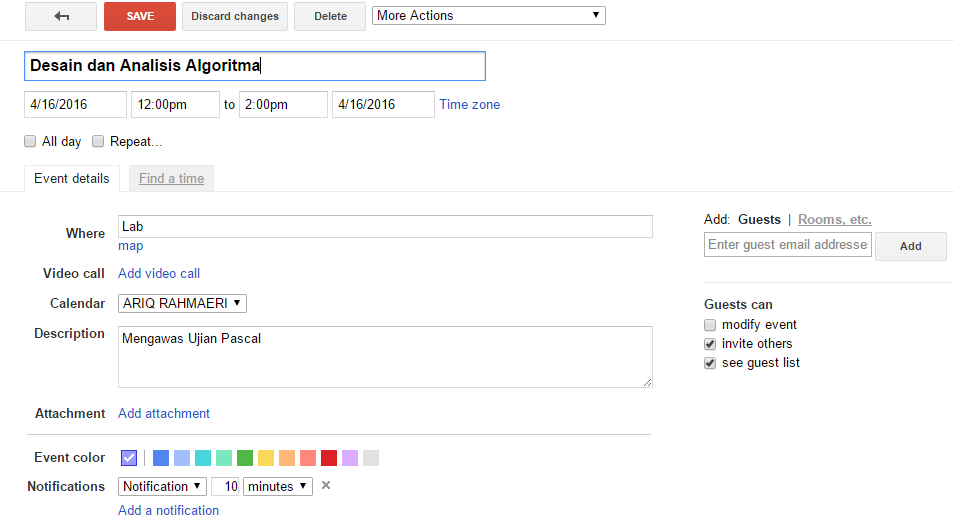
\includegraphics[scale=0.6]{Gambar/hasilGCFilter2}
			\caption{Hasil import file yang di filter ke Google Calendar bagian 2 }
			\label{fig:hasilGCFilter2}
			\end{figure}
			
	
			\begin{figure}[H]
			\centering
			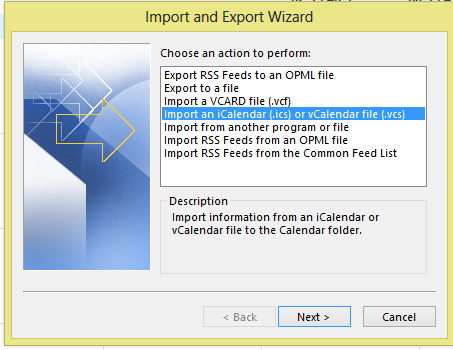
\includegraphics[scale=0.8]{Gambar/importOutlook}
			\caption{\textit{Import} file iCal yang telah di filter kedalam MS Outlook }
			\label{fig:importOutlookFilter}
			\end{figure}
		
			\begin{figure}[H]
			\centering
			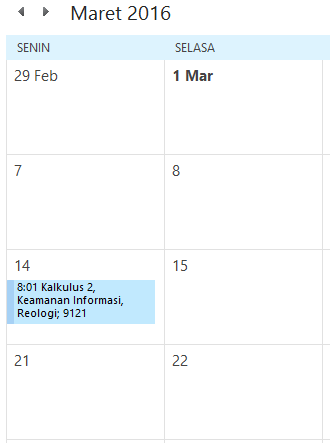
\includegraphics[scale=0.8]{Gambar/hasilOutlook2}
			\caption{File iCal yang telah di filter berada pada kalender MS Outlook }
			\label{fig:hasilOutlookFilter2}
			\end{figure}
			
			\begin{figure}[H]
			\centering
			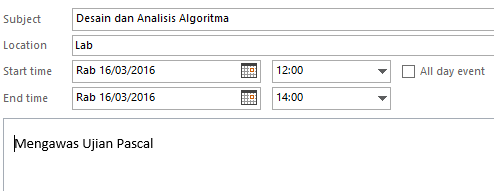
\includegraphics[scale=0.8]{Gambar/hasilOutlookFilter}
			\caption{File hasil filter dapat dibuka di MS Outlook }
			\label{fig:hasilOutlookFilter}
			\end{figure}
			


\subsection{Pengujian Eksperimental}
Pengujian eksperimental merupakan pengujian yang dilakukan dengan melibatkan skenario yang bersifat eksperimental. Pengujian ini ditujukan untuk melihat reaksi program menerima berbagai kejadian. Selain itu, file uji \ref{fig:formatBaru} pada pengujian eksperimental ini merupakan format file baru yang dikeluarkan TU FTIS untuk 2016. Berikut hasil pengujiannya :
\begin{table}[H]
	\centering
		\caption{Tabel hasil pengujian eksperimental}
		\label{tab:eksperimental}
		\begin{tabular}{ | p{4cm} | p{4cm} | p{4cm} | }
			\hline
				Hal yang diuji & Hasil yang diharapkan & Hasil \\ \hline
				Browse file excel & PL dapat melakukan browse file excel & Berhasil \ref{fig:browseFile}\\ \hline
				Path file excel & PL dapat menangkap alamat file dari \textit{input file} excel & Berhasil \ref{fig:pathFile} \\ \hline
				Memasukan file yang bukan excel & PL mengeluarkan notifikasi kesalahan file \textit{input} & Berhasil \ref{fig:eksperimental2} \\ \hline
				Menampilkan Jadwal ke layar & PL menampilkan ke layar file excel yang telah dibaca & Tidak berhasil Karena format tahun pada file excel jadwal baru menggunakan tanda '`' untuk menandakan tahun (`16). Sehingga, \textit{output} yang dikeluarkan PL berupa notifikasi kesalahan format  \ref{fig:eksperimental} \\ \hline
		\end{tabular}
\end{table}

Berikut ini merupakan gambar hasil pengujian eksperimental : 

			\begin{figure}[H]
			\centering
			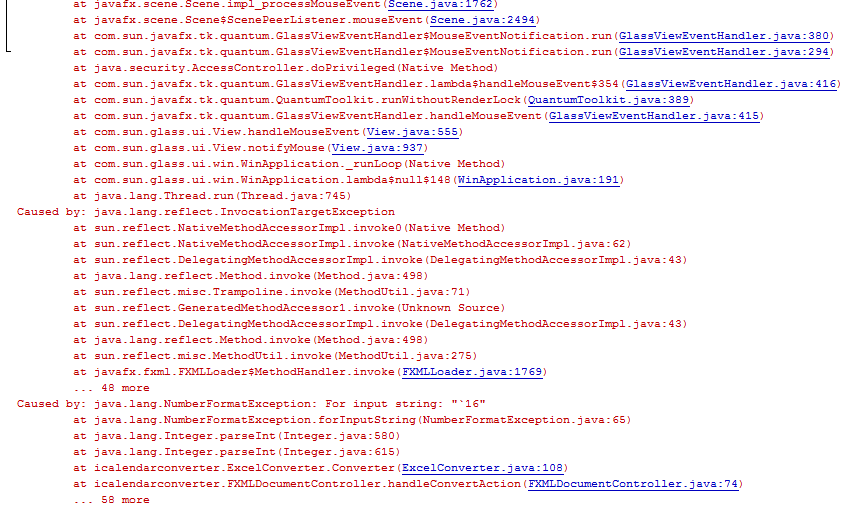
\includegraphics[scale=0.6]{Gambar/eksperimental}
			\caption{\textit{Output} PL pada pengujian eksperimental }
			\label{fig:eksperimental}
			\end{figure}
	

			\begin{figure}[H]
			\centering
			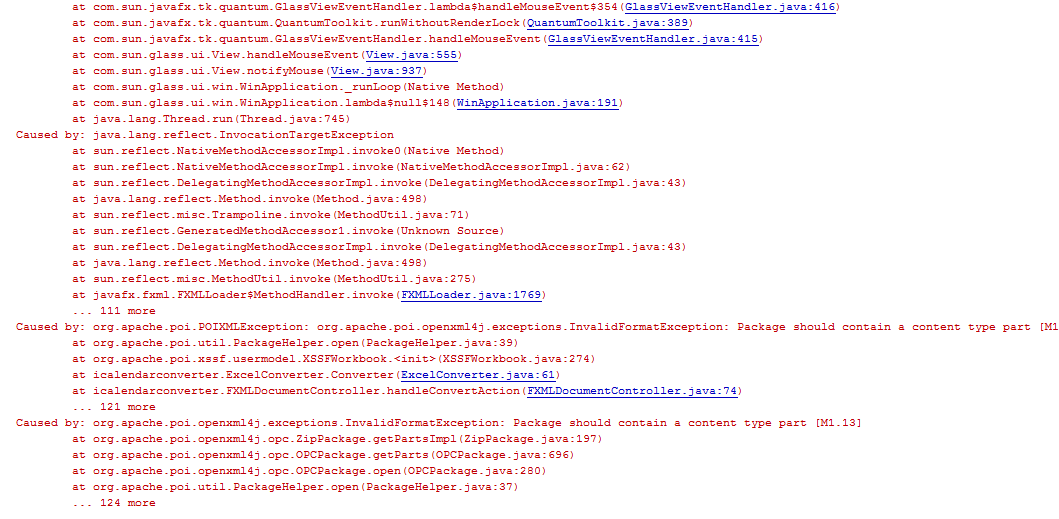
\includegraphics[scale=0.6]{Gambar/eksperimental2}
			\caption{\textit{Output} PL pada pengujian eksperimental dari file \textit{input} yang bukan excel}
			\label{fig:eksperimental2}
			\end{figure}		


Berdasarkan hasil pengujian tersebut maka dilakukan perubahan pada cara membaca PL sehingga dapat membaca kedua file excel, baik format lama maupun format baru yang dikeluarkan TU FTIS. Kelas ExcelConverter sebelum revisi dapat dilihat pada \ref{lst:ExcelConverterLama}. Berikut hasil pengujian setelah revisi : 

\begin{table}[H]
	\centering
		\caption{Tabel hasil pengujian eksperimental setelah revisi}
		\label{tab:eksperimental}
		\begin{tabular}{ | p{4cm} | p{4cm} | p{4cm} | }
			\hline
				Hal yang diuji & Hasil yang diharapkan & Hasil \\ \hline
				Browse file excel & PL dapat melakukan browse file excel & Berhasil \ref{fig:browseFile}\\ \hline
				Path file excel & PL dapat menangkap alamat file dari \textit{input file} excel & Berhasil \ref{fig:pathFile} \\ \hline
				Memasukan file yang bukan excel & PL menggunakan \textit{extension filter} sehingga file bukan excel tidak dapat menjadi file \textit{input} & Berhasil \ref{fig:filterExtension} \\ \hline
				Menampilkan Jadwal ke layar & PL menampilkan ke layar file excel yang telah dibaca & Berhasil \ref{fig:jadwalKeLayarEksperimental} \\ \hline
				Konversi ke iCal & PL dapat mengkonversi jadwal yang diseleksi pengguna kedalam iCalendar & Berhasil \ref{fig:konversiiCalEksperimental} \\ \hline
				Filter nama dosen & PL dapat menampilkan nama dosen yang telah di filter, sesuai yang di yang dimasukkan oleh pengguna pada \textit{textbox} filter & Berhasil \ref{fig:filterDosen} \\ \hline
				Hasil Filter dapat dikonversi ke iCal & Hasil Filter pada PL dan diseleksi oleh pengguna, dapat di konversikan kedalam iCal & Berhasil \ref{fig:filterKonvertiCaEksperimentall} \\ \hline
				\textit{Import} Google Calendar & Hasil konversi PL dapat di masukan kedalam Google Calendar & Berhasil \ref{fig:hasilGCEksperimental} \\ \hline
				Dapat dibuka di Outlook & Hasil konversi PL dapat di buka di Outlook & Berhasil  \ref{fig:hasilOutlookEksperimental2}\\ \hline
				Hasil filter dapat di \textit{import} Google Calendar & Hasil filter konversi PL dapat di masukan kedalam Google Calendar & Berhasil \ref{fig:hasilGCFilterEksperimental} \\ \hline
				Hasil filter Dapat dibuka di Outlook & Hasil filter konversi PL dapat di buka di Outlook & Berhasil \ref{fig:hasilOutlookFilterEksperimental2} \\ \hline
		\end{tabular}
\end{table}

Berikut merupakan tampilan dari hasil pengujian menggunakan file excel dengan format baru \ref{fig:formatBaru} :

		\begin{figure}[H]
		\centering
		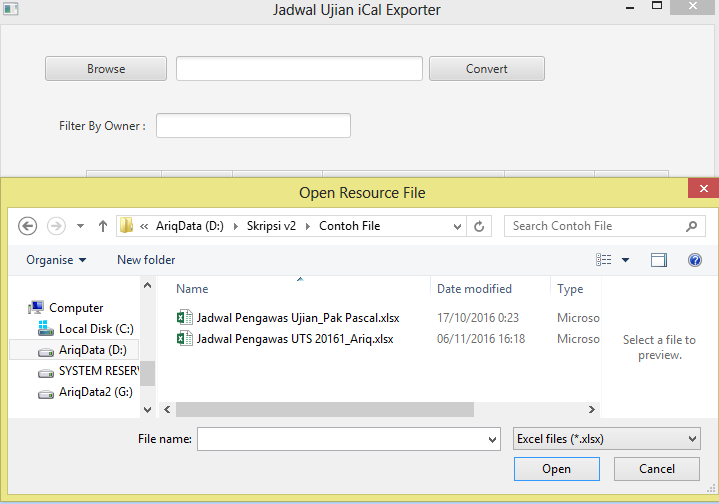
\includegraphics[scale=0.7]{Gambar/filterExtension}
		\caption{PL memfilter ekstensi file excel yang akan dimasukkan}
		\label{fig:filterExtension}
		\end{figure}
	 
		\begin{figure}[H]
		\centering
		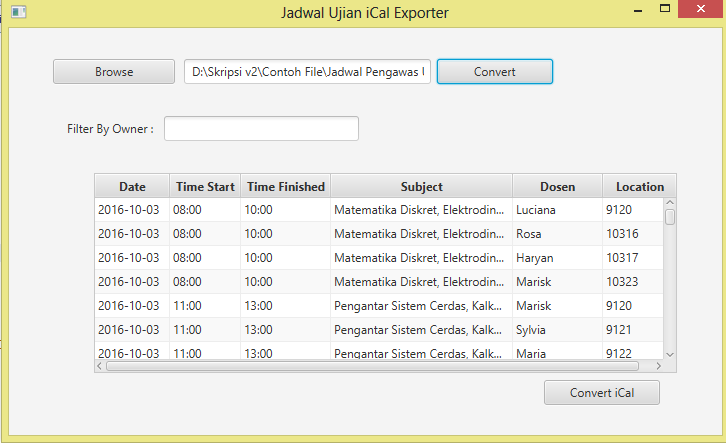
\includegraphics[scale=0.7]{Gambar/jadwalKeLayarEksperimental}
		\caption{PL menampilkan jadwal ke layar}
		\label{fig:jadwalKeLayarEksperimental}
		\end{figure}
 
		\begin{figure}[H]
		\centering
		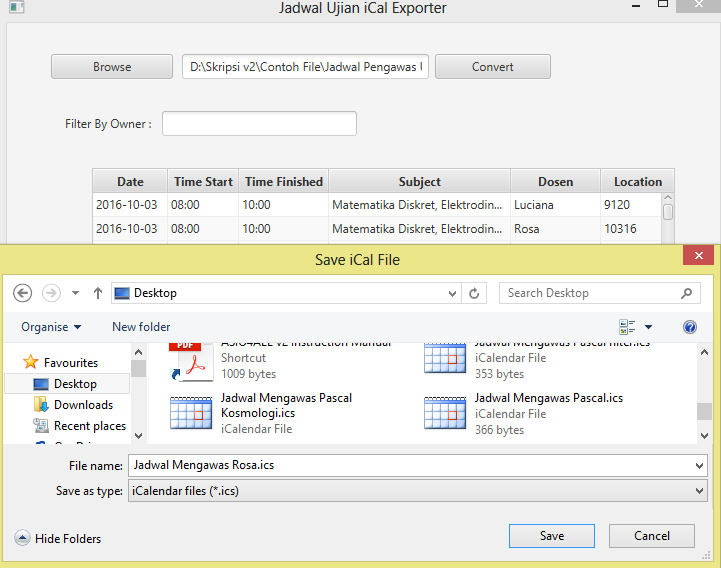
\includegraphics[scale=0.6]{Gambar/konversiiCalEksperimental}
		\caption{PL mengkonversi jadwal ke format iCal}
		\label{fig:konversiiCalEksperimental}
		\end{figure}
		
		\begin{figure}[H]
		\centering
		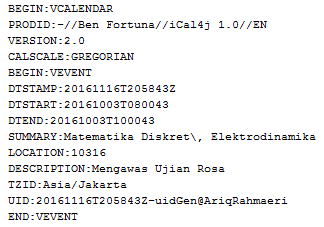
\includegraphics[scale=0.8]{Gambar/fileiCalEksperimental}
		\caption{File iCal}
		\label{fig:fileiCalEksperimental}
		\end{figure}
	
		\begin{figure}[H]
		\centering
		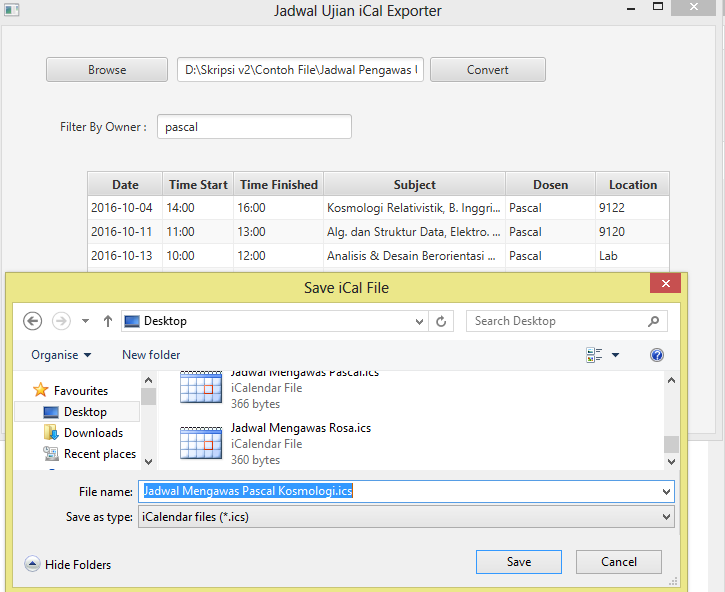
\includegraphics[scale=0.6]{Gambar/filterKonvertiCalEksperimental}
		\caption{Hasil pengujian convert hasil filter kedalam iCal}
		\label{fig:filterKonvertiCaEksperimentall}
		\end{figure}
		
		\begin{figure}[H]
		\centering
		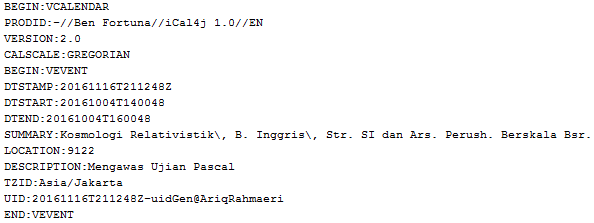
\includegraphics[scale=0.7]{Gambar/fileiCalFilterEksperimental}
		\caption{File iCal Filter}
		\label{fig:fileiCalFilterEksperimental}
		\end{figure}
	 
		\begin{figure}[H]
		\centering
		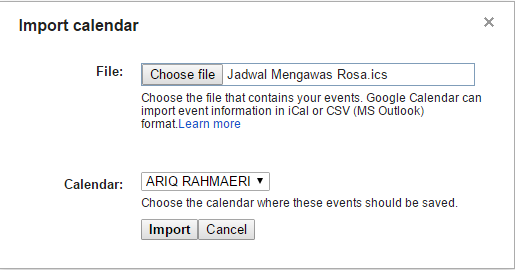
\includegraphics[scale=0.8]{Gambar/importGCEksperimental}
		\caption{Hasil pengujian import kedalam Google Calendar}
		\label{fig:importGC}
		\end{figure}
		
		\begin{figure}[H]
		\centering
		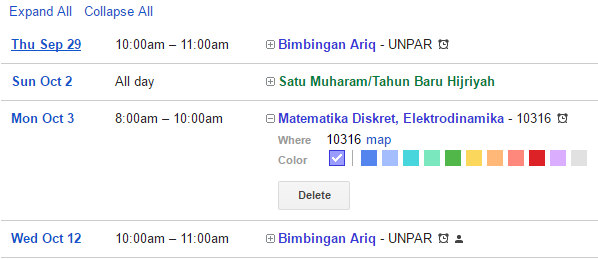
\includegraphics[scale=0.7]{Gambar/hasilGCEksperimental}
		\caption{Hasil import ke Google Calendar}
		\label{fig:hasilGCEksperimental}
		\end{figure}
		
		\begin{figure}[H]
		\centering
		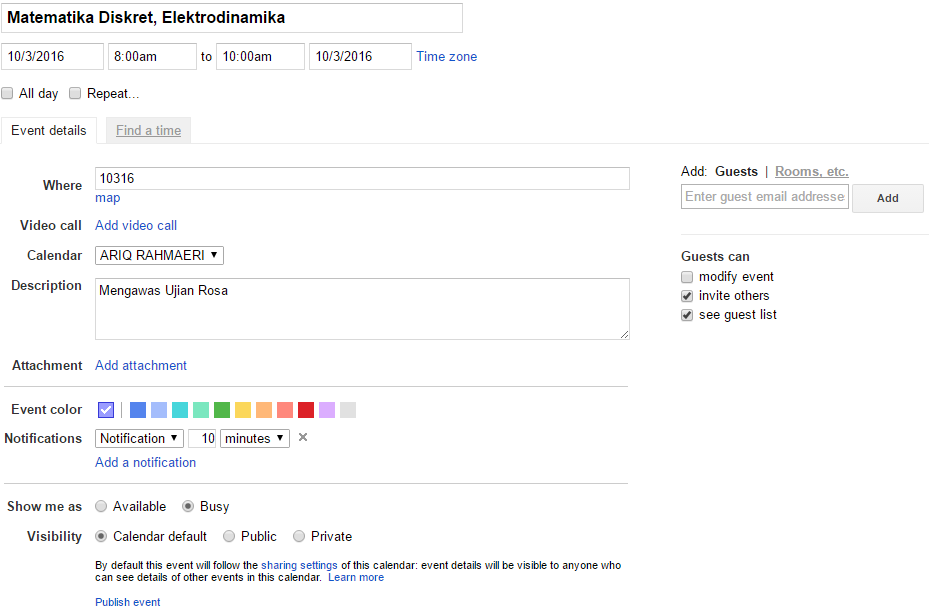
\includegraphics[scale=0.5]{Gambar/hasilGCEksperimental2}
		\caption{Hasil import ke Google Calendar bagian 2 }
		\label{fig:hasilGCEksperimental2}
		\end{figure}
		
	
			\begin{figure}[H]
			\centering
			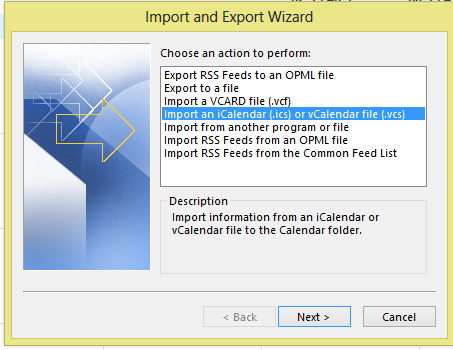
\includegraphics[scale=0.8]{Gambar/importOutlook}
			\caption{\textit{Import} file iCal kedalam MS Outlook }
			\label{fig:importOutlook}
			\end{figure}
		
			\begin{figure}[H]
			\centering
			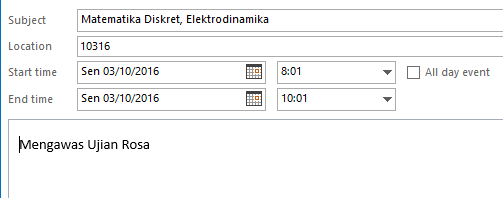
\includegraphics[scale=0.8]{Gambar/hasilOutlookEksperimental2}
			\caption{File hasil Konversi dapat dibuka di MS Outlook}
			\label{fig:hasilOutlookEksperimental2}
			\end{figure}
			
			\begin{figure}[H]
			\centering
			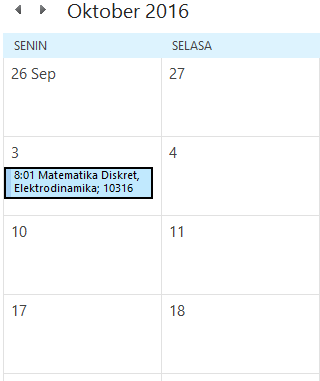
\includegraphics[scale=0.8]{Gambar/hasilOutlookEksperimental}
			\caption{File hasil Konversi berada pada kalender MS Outlook}
			\label{fig:hasilOutlookEksperimental}
			\end{figure}
		
	
			\begin{figure}[H]
			\centering
			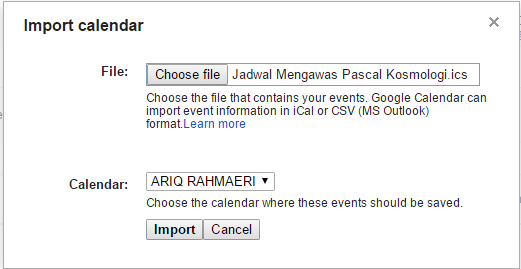
\includegraphics[scale=0.8]{Gambar/importGCFilterEksperimental}
			\caption{Hasil pengujian import file yang di filter kedalam Google Calendar }
			\label{fig:importGCFilterEksperimental}
			\end{figure}
			
			\begin{figure}[H]
			\centering
			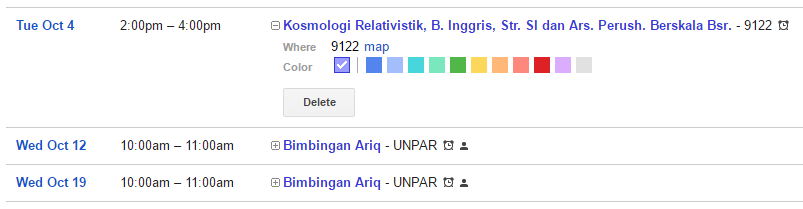
\includegraphics[scale=0.7]{Gambar/hasilGCFilterEksperimental}
			\caption{Hasil import file yang di filter ke Google Calendar}
			\label{fig:hasilGCFilterEksperimental}
			\end{figure}
			
			\begin{figure}[H]
			\centering
			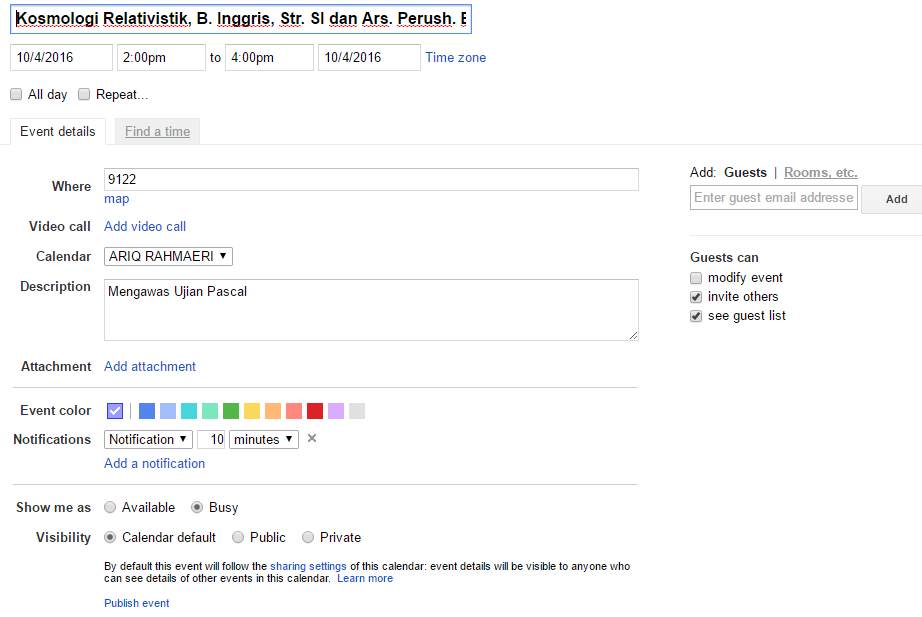
\includegraphics[scale=0.6]{Gambar/hasilGCFilterEksperimental2}
			\caption{Hasil import file yang di filter ke Google Calendar bagian 2 }
			\label{fig:hasilGCFilterEksperimental2}
			\end{figure}
			
		
			\begin{figure}[H]
			\centering
			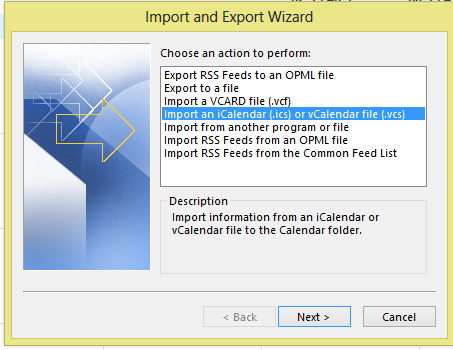
\includegraphics[scale=0.8]{Gambar/importOutlook}
			\caption{\textit{Import} file iCal yang telah di filter kedalam MS Outlook }
			\label{fig:importOutlookFilter}
			\end{figure}
		
			\begin{figure}[H]
			\centering
			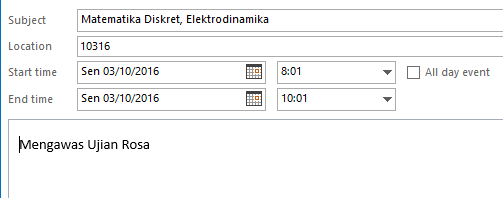
\includegraphics[scale=0.8]{Gambar/hasilOutlookEksperimental2}
			\caption{File hasil filter dapat dibuka di MS Outlook}
			\label{fig:hasilOutlookFilterEksperimental2}
			\end{figure}
			
			\begin{figure}[H]
			\centering
			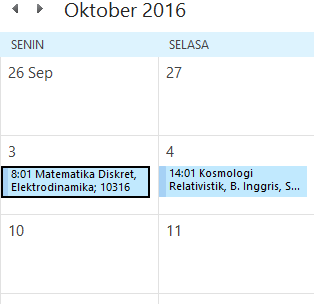
\includegraphics[scale=0.8]{Gambar/hasilOutlookFilterEksperimental}
			\caption{File iCal yang telah di filter berada pada kalender MS Outlook}
			\label{fig:hasilOutlookFilter}
			\end{figure}
			


Selain menguji pada sistem operasi windows, PL juga diuji pada sistem operasi Mac OS. Pada kesempatan kali ini PL diuji kinerjanya dalam OS X. PL diuji pada Macbook Pa Pascal dengan skenario yang sama pada sistem operasi windows. Berikut hasil pengujiannya.
\begin{table}[H]
	\centering
		\caption{Tabel hasil pengujian pada OS X}
		\label{tab:eksperimental}
		\begin{tabular}{ | p{4cm} | p{4cm} | p{4cm} | }
			\hline
				Hal yang diuji & Hasil yang diharapkan & Hasil \\ \hline
				Browse file excel & PL dapat melakukan browse file excel & Berhasil \ref{fig:BrowseonMac} \ref{fig:BrowseDatabaruonMac}\\ \hline
				Menampilkan Jadwal ke layar & PL menampilkan ke layar file excel yang telah dibaca & Berhasil \ref{fig:MenampilkankelayaronMac}  \ref{fig:MenampilkankelayarDatabaruonMac}\\ \hline
				Konversi ke iCal & PL dapat mengkonversi jadwal yang diseleksi pengguna kedalam iCalendar & Berhasil \ref{fig:Save-iCal-on-Mac} \ref{fig:Save-iCal-Data-Baru-on-Mac} \\ \hline
				Hasil Filter dapat dikonversi ke iCal & Hasil Filter pada PL dan diseleksi oleh pengguna, dapat di konversikan kedalam iCal & Berhasil \ref{fig:Save-iCal-Filter-on-Mac} \ref{fig:Save-iCal-Data-Baru-Filter-on-Mac}  \\ \hline
				Import iCalendar Mac & Hasil konversi PL dapat di masukan kedalam iCalendar pada OS X & Berhasil \ref{fig:Hasil-Import-2-on-Mac} \ref{fig:Hasil-iCal-Data-Baru-on-Mac} \\ \hline
				Hasil filter dapat di \textit{import} Google Calendar & Hasil filter konversi PL dapat di masukan kedalam Google Calendar & Berhasil \ref{fig:Hasil-Import-Filter-2-on-Mac} \ref{fig:Hasil-iCal-Data-Baru-Filter}\\ \hline
		\end{tabular}
\end{table} 
	Berikut tampilan dari hasil pengujian PL pada OS X :

		\begin{figure}[H]
			\centering
			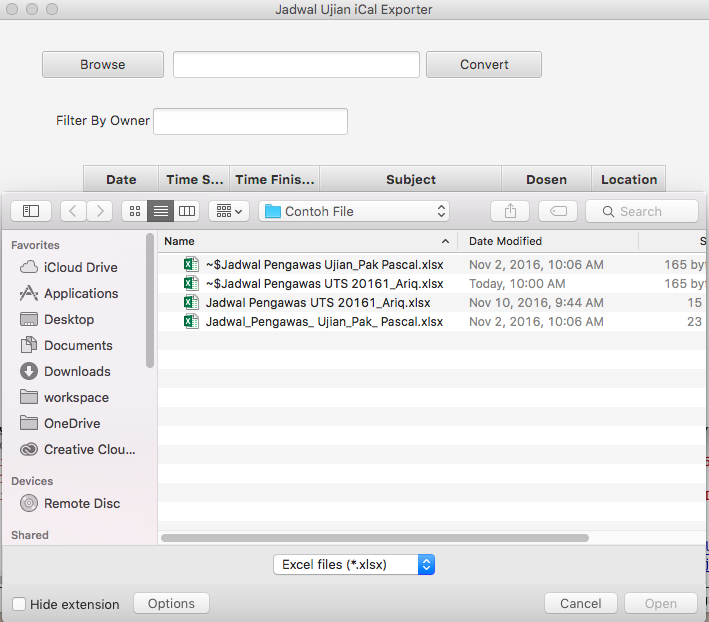
\includegraphics[scale=0.5]{Gambar/BrowseonMac}
			\caption{Hasil pengujian \textit{browse} pada OS X dengan \textit{file input} data lama}
			\label{fig:BrowseonMac}
			\end{figure}
		
		
		\begin{figure}[H]
			\centering
			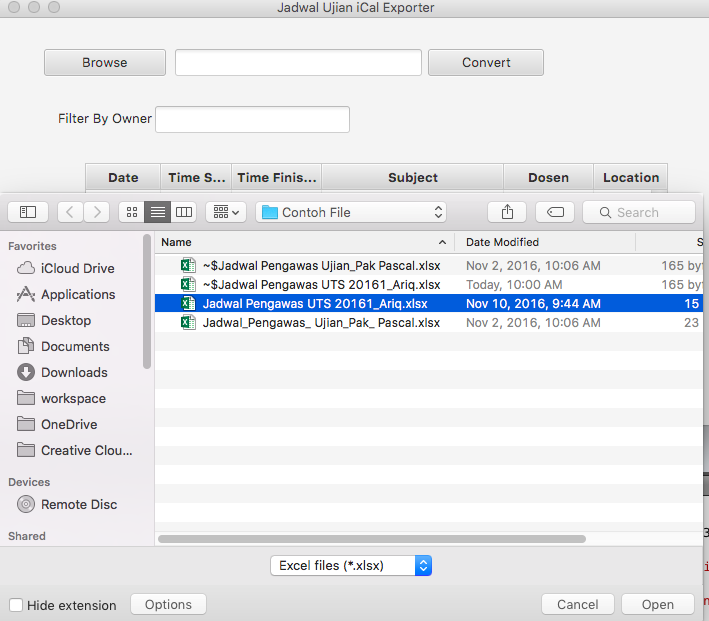
\includegraphics[scale=0.5]{Gambar/BrowseDatabaruonMac}
			\caption{Hasil pengujian \textit{browse} pada OS X dengan \textit{file input} data baru}
			\label{fig:BrowseDatabaruonMac}
			\end{figure}
			
		\begin{figure}[H]
			\centering
			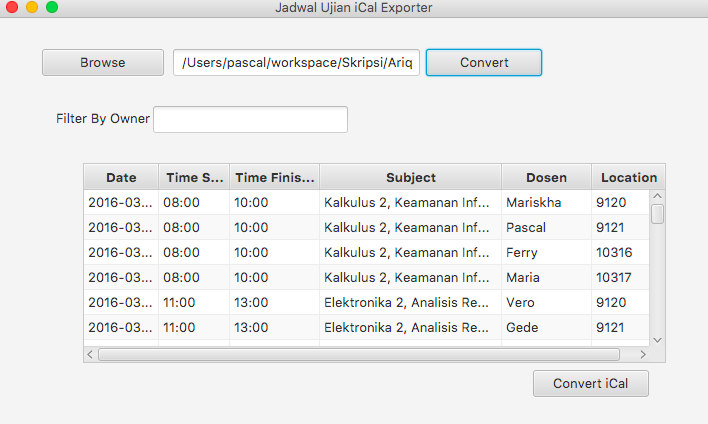
\includegraphics[scale=0.5]{Gambar/Menampilkan-ke-layar-on-Mac}
			\caption{Hasil pengujian menampilkan ke layar pada OS X dengan \textit{file input} data lama}
			\label{fig:MenampilkankelayaronMac}
			\end{figure}
		
		\begin{figure}[H]
			\centering
			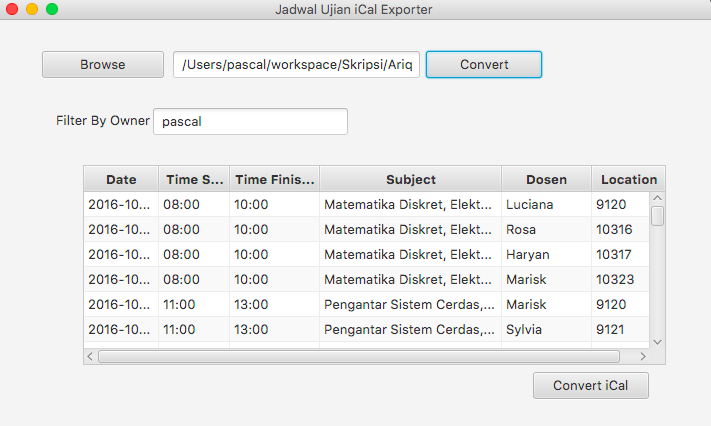
\includegraphics[scale=0.5]{Gambar/Menampilkan-ke-Layar-Data-baru-on-Mac}
			\caption{Hasil pengujian menampilkan ke layar pada OS X dengan \textit{file input} data baru}
			\label{fig:MenampilkankelayarDatabaruonMac}
			\end{figure}
			
		\begin{figure}[H]
			\centering
			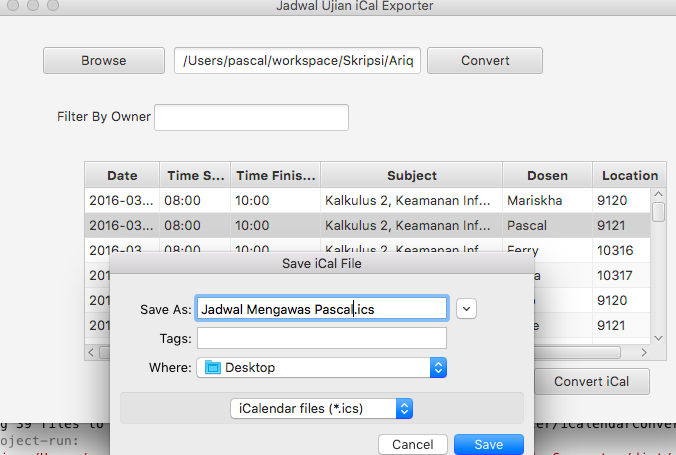
\includegraphics[scale=0.5]{Gambar/Save-iCal-on-Mac}
			\caption{Hasil pengujian menyimpan file iCal pada OS X dengan \textit{file input} data lama}
			\label{fig:Save-iCal-on-Mac}
			\end{figure}
		
		\begin{figure}[H]
			\centering
			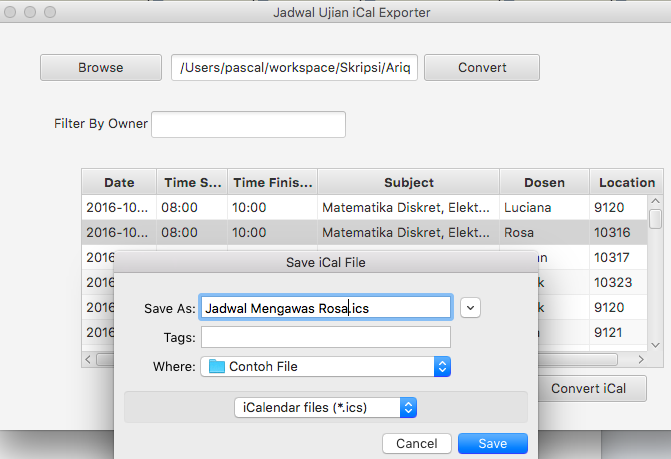
\includegraphics[scale=0.5]{Gambar/Save-iCal-Data-Baru-on-Mac}
			\caption{Hasil pengujian menyimpan file iCal pada OS X dengan \textit{file input} data baru}
			\label{fig:Save-iCal-Data-Baru-on-Mac}
			\end{figure}
		
		\begin{figure}[H]
			\centering
			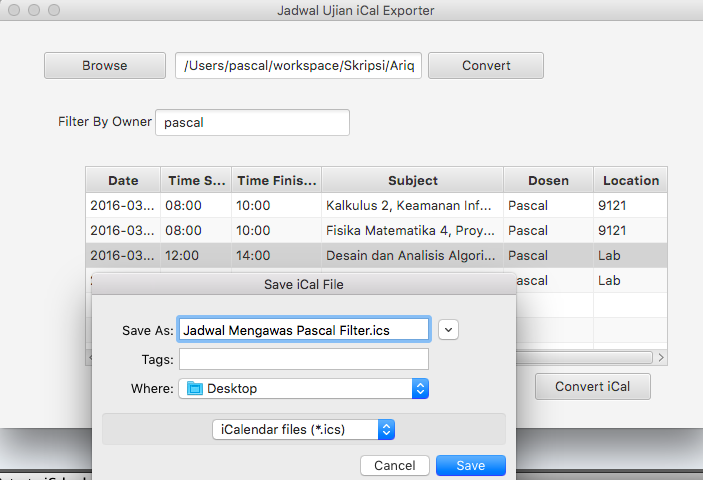
\includegraphics[scale=0.5]{Gambar/Save-iCal-Filter-on-Mac}
			\caption{Hasil pengujian menyimpan file iCal yang telah difilter pada OS X dengan \textit{file input} data lama}
			\label{fig:Save-iCal-Filter-on-Mac}
			\end{figure}
		
		\begin{figure}[H]
			\centering
			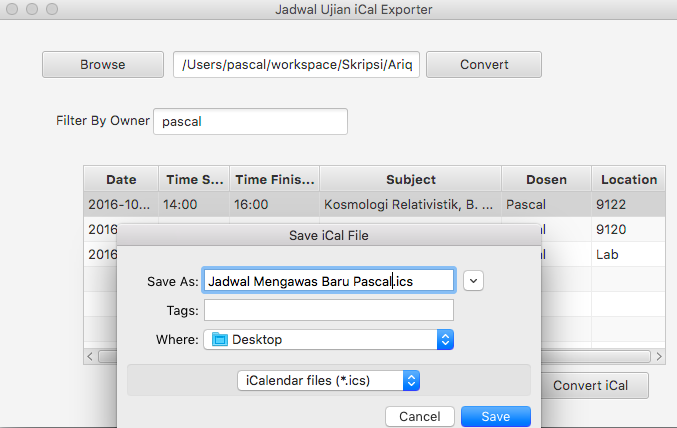
\includegraphics[scale=0.5]{Gambar/Save-iCal-Data-Baru-Filter-on-Mac}
			\caption{Hasil pengujian menyimpan file iCal yang telah difilter pada OS X dengan \textit{file input} data baru}
			\label{fig:Save-iCal-Data-Baru-Filter-on-Mac}
			\end{figure}
			
			\begin{figure}[H]
			\centering
			\includegraphics[scale=0.5]{Gambar/Import-Jadwal-on-Mac}
			\caption{Hasil pengujian \textit{import} iCalendar pada OS X dengan \textit{file input} data lama}
			\label{fig:Import-Jadwal-on-Mac}
			\end{figure}
			
			\begin{figure}[H]
			\centering
			\includegraphics[scale=0.5]{Gambar/Import-Jadwal-2-on-Mac}
			\caption{Notifikasi destinasi kalendar pada OS X dengan \textit{file input} data lama}
			\label{fig:Import-Jadwal-2-on-Mac}
			\end{figure}
			
			\begin{figure}[H]
			\centering
			\includegraphics[scale=0.4]{Gambar/Hasil-import-on-Mac}
			\caption{Tampilan iCalendar pada OS X dengan \textit{file input} data lama}
			\label{fig:Hasil-import-on-Mac}
			\end{figure}
			
			\begin{figure}[H]
			\centering
			\includegraphics[scale=0.4]{Gambar/Hasil-Import-2-on-Mac}
			\caption{Tampilan iCalendar bagian 2 pada OS X dengan \textit{file input} data lama}
			\label{fig:Hasil-Import-2-on-Mac}
			\end{figure}
			
			\begin{figure}[H]
			\centering
			\includegraphics[scale=0.3]{Gambar/Hasil-iCal-Data-Baru-on-Mac}
			\caption{Tampilan iCalendar  pada OS X dengan \textit{file input} data baru}
			\label{fig:Hasil-iCal-Data-Baru-on-Mac}
			\end{figure}
			
			\begin{figure}[H]
			\centering
			\includegraphics[scale=0.4]{Gambar/Hasil-Import-Filter-on-Mac}
			\caption{Tampilan hasil filter pada OS X dengan \textit{file input} data lama}
			\label{fig:Hasil-Import-Filter-on-Mac}
			\end{figure}
			
			\begin{figure}[H]
			\centering
			\includegraphics[scale=0.4]{Gambar/Hasil-Import-Filter-2-on-Mac}
			\caption{Tampilan hasil filter bagian 2 pada OS X dengan \textit{file input} data lama}
			\label{fig:Hasil-Import-Filter-2-on-Mac}
			\end{figure}
			
			Hasil-iCal-Data-Baru-Filter
			\begin{figure}[H]
			\centering
			\includegraphics[scale=0.4]{Gambar/Hasil-iCal-Data-Baru-Filter}
			\caption{Tampilan hasil filter pada OS X dengan \textit{file input} data baru}
			\label{fig:Hasil-iCal-Data-Baru-Filter}
			\end{figure}
			